%To compile, run the following command:
%   latexmk -pdf latex_template.tex 
%
% To edit, you can use your favorite text editor or LaTeX editors such as:
%   Texmaker and TeXworks.
%
% To set up your own TeX system, you can install TeX Live. See:
% https://www.tug.org/texlive/


% For a recent install of texlive on Ubuntu 18.04 that is adequate for
% compiling this file, I used the following commands:
%
% sudo apt install texlive-latex-base
% sudo apt install texlive-latex-extra
% sudo apt install texlive-science

\documentclass[letterpaper,12pt]{article}

\usepackage[margin=1in]{geometry}
\usepackage{amsmath,amsthm,amsfonts,amssymb}
\usepackage{mathtools}
\usepackage{algorithm,algpseudocode}
\usepackage{algorithm}
\usepackage{algpseudocode}
\usepackage{hyperref}
\usepackage{graphicx}
\usepackage{array}
\usepackage{subcaption}

\theoremstyle{remark}
\newtheorem{claim}{Claim}

\DeclarePairedDelimiter\abs{\lvert}{\rvert}
\DeclarePairedDelimiter\floor{\lfloor}{\rfloor}
\DeclarePairedDelimiter\ceiling{\lceil}{\rceil}

\begin{document}

\title{Lab 2: KMeans with CUDA: \\
\large 
Performance analysis and detailed approach
   }


\date{\today}
\author{Qiying Wu}
\maketitle





\section*{Abstract }

 This report presents the implementation and performance analysis of the KMeans clustering algorithm using both CPU and GPU parallelism. The goal of this lab is to explore the benefits of GPU programming through the use of CUDA and Thrust libraries. The KMeans algorithm, commonly used for unsupervised machine learning, was implemented in four variations: a sequential CPU version, a basic CUDA version, an optimized CUDA version utilizing shared memory, and a high-level parallel implementation using the Thrust library.

I have conducted performance evaluations across datasets of varying sizes and dimensions, comparing the execution times and speedups of each implementation. The results show significant improvements in the CUDA-based versions, with the shared memory implementation providing the fastest runtime, surpassing both the sequential and Thrust implementations. We also analyze the effect of data transfer overhead between the CPU and GPU and examine the impact of non-deterministic behavior introduced by atomic operations in the CUDA implementations. The analysis highlights the trade-offs between ease of implementation and performance optimization, with the CUDA shared memory version achieving the best speedup compared to the sequential approach. 


\section*{Introduction }
KMeans is one of the most widely used clustering algorithms in machine learning, particularly for unsupervised tasks where the goal is to group data points into cohesive clusters based on feature similarity. The algorithm iteratively assigns data points to clusters and updates the cluster centroids until convergence. Despite its simplicity, KMeans is computationally expensive, especially for large datasets and high-dimensional data, making it an ideal candidate for parallelization.

The purpose of this lab is to explore the performance benefits of using GPUs for parallel computation through the implementation of KMeans using CUDA and the Thrust library. GPU programming enables significant speedups by exploiting data parallelism, allowing thousands of threads to run concurrently, which can greatly reduce the execution time of computationally intensive tasks like KMeans. 

In this lab, we implement and compare four different versions of the KMeans algorithm:
\begin{itemize}
    \item \textbf{Sequential CPU Implementation:} A basic, single-threaded version of KMeans executed on the CPU.
    \item \textbf{CUDA Basic Implementation:} A parallel GPU version of KMeans using CUDA for computation.
    \item \textbf{CUDA with Shared Memory:} An optimized GPU version that utilizes CUDA's shared memory to reduce global memory access latency and improve performance.
    \item \textbf{Thrust Implementation:} A high-level parallel implementation using NVIDIA's Thrust library, which abstracts thread management and allows for efficient use of parallel primitives.
\end{itemize}

This report presents the design and implementation of these different approaches, along with performance analyses based on their execution times for various datasets. We also discuss the challenges encountered during the optimization process, including memory management and non-deterministic behavior caused by atomic operations in CUDA. By comparing the performance of these implementations, we aim to highlight the trade-offs between different levels of abstraction in GPU programming and the impact of hardware-level optimizations on the performance of parallel algorithms like KMeans.



\section{Hardware and Software Specifications}

\small
The following details describe the GPU hardware available on the system, obtained using the \texttt{nvidia-smi} tool, all testing done in codio.

\subsection{General Information}
\begin{itemize}
    \item \textbf{GPU Model:} Tesla T4
    \item \textbf{Total GPU Memory:} 15,360 MiB (15 GB)
    \item \textbf{Driver Version:} 550.90.07
    \item \textbf{CUDA Version:} 12.4
\end{itemize}

\subsection{CUDA Core Calculation}
\begin{itemize}
    \item The Tesla T4 GPU has \textbf{40 streaming multiprocessors (SMs)}.
    \item Each SM contains \textbf{64 CUDA cores}.
    \item Therefore, the total number of CUDA cores is:
    \[
    \text{Total CUDA Cores} = 40 \, \text{SMs} \times 64 \, \text{CUDA cores per SM} = 2,560 \, \text{CUDA cores}
    \]
\end{itemize}

\subsection{CPU Hardware and Operating System}
\begin{itemize}
    \item \textbf{CPU Model:} Intel Core i7-9700K (8 cores)
    \item \textbf{CPU Clock Speed:} 3.6 GHz
    \item \textbf{Operating System:} Ubuntu 20.04
\end{itemize}
\normalsize




\subsection{Summary}
The Tesla T4 GPU is a data-center grade GPU with 15 GB of memory, optimized for tasks such as machine learning and high-performance computing. The GPU contains a total of 2,560 CUDA cores, making it capable of efficiently handling parallel computations. The system is ready to handle computationally intensive tasks with persistence mode enabled to ensure low-latency usage during repeated tasks.


\section{Algorithm and Implementations}
For all the different implementations, I am using the following kmeans algorithm, with slightly difference.
\begin{algorithm} 
\caption{KMeans Algorithm}\label{kmeans}
\begin{algorithmic}[1]
\State \textbf{Input:} Data points, $k$ centroids, max iterations, threshold
\State \textbf{Output:} Cluster assignments and centroids

\State \textbf{Initialization:}
\State Initialize $k$ centroids randomly
\State Initialize labels and cluster sizes

\For{each iteration (up to max iterations)}
    \State \textbf{Step 1: Assignment}
    \For{each point $i$}
        \State Compute Euclidean distance to all centroids
        \State Assign point $i$ to the nearest centroid
    \EndFor

    \State \textbf{Step 2: Centroid Update}
    \State Reset centroids and cluster sizes
    \For{each point $i$}
        \State Add point $i$ to its assigned centroid
        \State Update cluster sizes
    \EndFor
    \State Normalize centroids by dividing by cluster sizes

    \State \textbf{Step 3: Convergence Check}
    \State Compute total shift of centroids OR per dimension convergence check
    
\EndFor
\end{algorithmic}
\end{algorithm}
\clearpage


The initialization of random centroid will be done by kmeans.cpp, before we call different implementations. The inpput and output are the same for all implementations.


\begin{enumerate}
    \item \textbf{Input:} Data points, $k$ centroids, maximum iterations, convergence threshold.
    \item \textbf{Output:} Final centroids and cluster labels.
\end{enumerate}

For running the respective implementations, the following command can be used:

\begin{verbatim}
./bin/kmeans -k 16 -t 1e-5 -i input/random-n2048-d16-c16.txt 
-m 2000 -s 8675309 -d 16 -c --use_cuda_gmem
\end{verbatim}

\begin{verbatim}
./bin/kmeans -k 16 -t 1e-5 -i input/random-n16384-d24-c16.txt 
-m 2000 -s 8675309 -d 24 -c --use_cuda_shmem
\end{verbatim}

\begin{verbatim}
./bin/kmeans -k 16 -t 1e-5 -i input/random-n65536-d32-c16.txt 
-m 2000 -s 8675309 -d 32 -c --use_cuda_thrust
\end{verbatim}

\textbf{Explanation of the command:}
\begin{itemize}
    \item \texttt{-k 16}: Specifies the number of clusters (16).
    \item \texttt{-t 1e-5}: Sets the convergence threshold to $1 \times 10^{-5}$.
    \item \texttt{-i input/random-n65536-d32-c16.txt}: Specifies the input file with 65536 points, 32 dimensions, and 16 clusters.
    \item \texttt{-m 2000}: Sets the maximum number of iterations to 2000.
    \item \texttt{-s 8675309}: Provides the random seed value (8675309).
    \item \texttt{-d 32}: Specifies the dimensionality of the input data (32).
    \item \texttt{-c}: Outputs the final centroids after the KMeans computation.
    \item \texttt{--use\_cpu}: Specifies that the sequential version of the algorithm should be used.
    \item \texttt{--use\_cuda\_shmem}: Specifies that the CUDA shared memory version of the algorithm should be used.
    \item \texttt{--use\_cuda\_gmem}: Specifies that the CUDA global memory version should be used.
    \item \texttt{--use\_thrust}: Specifies that the CUDA thrust library version should be used.

\end{itemize}

\clearpage
\subsection{Sequential CPU Implementation}
The sequential KMeans implementation I implemented follows the algorithm above, when it checks for convergence, instead of using a total shift across dimensions, it performs a per-dimension convergence check to ensure finer control over the convergence criteria. The algorithm iterates until all centroid shifts are below a defined threshold or the maximum number of iterations is reached. This method ensures stability in each feature dimension before stopping.


\subsection{CUDA Basic Implementation (Global Memory)}
In the CUDA implementation, each data point and centroid computation was parallelized using CUDA threads. Kernels were designed to compute the distances between points and centroids, assign labels, and update centroids. The implementation includes memory transfers between host (CPU) and device (GPU), which contributes to the overall runtime.


\begin{enumerate}
    \item \textbf{Initialization:}
    \begin{itemize}
        \item Allocate memory for points, centroids, labels, cluster sizes, and changes on the device (GPU).
        \item Copy data points and initial centroids from the host (CPU) to the device (GPU).
        \item Initialize cluster sizes and old centroids on the device.
    \end{itemize}

    \item \textbf{Iterative Process:} For each iteration (up to maximum iterations):
    \begin{enumerate}
        \item \textbf{Assign Points to Nearest Centroid:}
        \begin{itemize}
            \item Launch a CUDA kernel to compute the distance between each point and all centroids.
            \item Assign each point to its nearest centroid in parallel.
        \end{itemize}
        
        \item \textbf{Compute New Centroids:}
        \begin{itemize}
            \item Reset centroids and cluster sizes in global memory.
            \item Launch a CUDA kernel to sum the points assigned to each centroid, using atomic operations to update the centroids and cluster sizes.
        \end{itemize}
        
        \item \textbf{Normalize Centroids:}
        \begin{itemize}
            \item Launch a CUDA kernel to normalize the centroids by dividing the accumulated values by the number of assigned points.
        \end{itemize}
        
        \item \textbf{Check for Convergence:}
        \begin{itemize}
            \item Copy centroids to old centroids for comparison.
            \item Launch a CUDA kernel to compute the difference between old and new centroids.
            \item Sum the total change in centroid positions using host-side code.
            \item If the total change is smaller than the threshold, terminate the loop.
        \end{itemize}
    \end{enumerate}
    
    \item \textbf{Final Step:}
    \begin{itemize}
        \item Copy the final centroids and labels from device (GPU) to host (CPU).
        \item Reshape the final centroids into a 2D vector for output.
    \end{itemize}
\end{enumerate}











\subsection{CUDA with Shared Memory}
The shared memory version of CUDA optimized memory access by reducing global memory accesses and using shared memory to store centroids, thus reducing latency and improving performance.

\begin{enumerate}
    \item \textbf{Initialization:}
    \begin{itemize}
        \item Allocate memory for points, centroids, labels, cluster sizes, and centroid change on the device (GPU).
        \item Copy data points and initial centroids from the host (CPU) to the device (GPU).
        \item Initialize cluster sizes and old centroids on the device.
        \item Set the size of shared memory to hold centroids for each block.
    \end{itemize}

    \item \textbf{Iterative Process:} For each iteration (up to maximum iterations):
    \begin{enumerate}
        \item \textbf{Assign Points to Nearest Centroid:}
        \begin{itemize}
            \item Load the centroids into shared memory for fast access.
            \item Launch a CUDA kernel to compute the distance between each point and all centroids using shared memory.
            \item Each thread assigns a point to its nearest centroid and updates the label array.
            \item Synchronize the threads after loading and calculating distances to ensure all threads have the updated data.
        \end{itemize}

        \item \textbf{Compute New Centroids:}
        \begin{itemize}
            \item Reset centroids and cluster sizes in global memory before computation.
            \item Launch a CUDA kernel that uses shared memory to accumulate point contributions to each centroid.
            \item Use atomic operations to update the centroids and cluster sizes in shared memory, reducing memory contention.
            \item Synchronize the threads after accumulation to ensure all updates to shared memory are completed.
        \end{itemize}

        \item \textbf{Normalize Centroids:}
        \begin{itemize}
            \item Launch a CUDA kernel to normalize the centroids by dividing the accumulated values by the number of points assigned to each centroid.
            \item Use shared memory to normalize each dimension of the centroids within each block, synchronizing the threads before writing to global memory.
        \end{itemize}

        \item \textbf{Check for Convergence:}
        \begin{itemize}
            \item Copy the current centroids to old centroids for the next iteration.
            \item Launch a CUDA kernel to compute the difference between the new and old centroids.
            \item Sum the changes across all centroids in host-side code to check if the total change is smaller than the defined threshold.
            \item If the total change is below the threshold, terminate the loop (i.e., convergence is achieved).
        \end{itemize}
    \end{enumerate}
    
    \item \textbf{Final Step:}
    \begin{itemize}
        \item Copy the final centroids and labels from the device (GPU) to the host (CPU).
        \item Reshape the final centroids into a 2D vector for output.
        \item Free all device memory used during the computation.
    \end{itemize}
\end{enumerate}









\subsection{Parallel GPU Implementation using Thrust}
The Thrust-based implementation used high-level parallel primitives such as \texttt{thrust::for\_each}, \texttt{thrust::reduce\_by\_key}, and \texttt{thrust::transform} to implement the KMeans algorithm. This method abstracts CUDA thread management but may not fully utilize GPU capabilities compared to direct CUDA kernel implementation.

\begin{enumerate}
    \item \textbf{Initialization:}
    \begin{itemize}
        \item Allocate memory for points, centroids, labels, and counts using Thrust device vectors on the GPU.
        \item Copy data points and initial centroids from the host (CPU) to the device (GPU) using Thrust.
        \item Initialize cluster counts and old centroids on the device.
        \item Create CUDA events to measure the execution time of the KMeans algorithm.
    \end{itemize}

    \item \textbf{Iterative Process:} For each iteration (up to maximum iterations):
    \begin{enumerate}
        \item \textbf{Assign Points to Nearest Centroid:}
        \begin{itemize}
            \item Launch a CUDA kernel to compute the distance between each point and all centroids, assigning each point to the nearest centroid.
            \item Store the resulting assignments (labels) in a device vector.
        \end{itemize}

        \item \textbf{Swap Old and New Centroids:}
        \begin{itemize}
            \item Copy the current centroids to the old centroids vector using Thrust's `copy` operation.
        \end{itemize}

        \item \textbf{Reset Centroids and Counts:}
        \begin{itemize}
            \item Reset the centroids and counts on the device to zero using Thrust's `fill` operation.
        \end{itemize}

        \item \textbf{Compute New Centroids:}
        \begin{itemize}
            \item Launch a CUDA kernel that uses atomic operations to sum the points assigned to each centroid and update the cluster sizes.
        \end{itemize}

        \item \textbf{Normalize Centroids:}
        \begin{itemize}
            \item Launch a CUDA kernel to normalize the centroids by dividing the accumulated sums by the number of points assigned to each centroid.
        \end{itemize}

        \item \textbf{Check for Convergence:}
        \begin{itemize}
            \item Launch a CUDA kernel to compute the squared differences between old and new centroids.
            \item Copy the differences back to the host and check for convergence by comparing the change in each centroid’s position to the given threshold.
            \item If the change is smaller than the threshold for all centroids, terminate the loop (convergence achieved).
        \end{itemize}
    \end{enumerate}
    
    \item \textbf{Final Step:}
    \begin{itemize}
        \item Copy the final centroids and labels from the device (GPU) to the host (CPU) using Thrust's `copy` operation.
        \item Reshape the final centroids into a 2D vector for output.
        \item Free all device memory and destroy the CUDA events.
    \end{itemize}
\end{enumerate}






\section{Baseline with cpu sequential}
The following table will display the sequential execution time.
\begin{table}[ht]
\centering
\caption{Execution Time (Total) for CPU Sequential Implementation and Input Sizes, baseline}
\begin{tabular}{|c|c|c|}
\hline
\textbf{Input Size} & \textbf{Total Time (ms)} & iter \\
\hline
random-n1-d1-c1      & 0.04 & 1 \\
random-n304-d21-c18  & 2.24 & 10 \\
random-n430-d12-c41  & 1.86 & 8 \\
random-n512-d19-c78  & 5.11 & 7 \\
random-n724-d18-c18  & 1.97 & 8 \\
random-n861-d31-c40  & 10.29 & 9 \\
random-n1024-d26-c84 & 25.20 & 11 \\
random-n2048-d16-c16 & 9.34 & 17 \\
random-n2048-d16-c16 & 9.28 & 17 \\
random-n2048-d16-c16 & 9.36 & 17 \\
random-n2896-d13-c85 & 41.10 & 13 \\
random-n3444-d13-c125 & 239.73 & 25 \\
random-n8192-d30-c109 & 330.85 & 11 \\
random-n9741-d10-c25  & 147.66 & 55 \\
random-n9741-d16-c44  & 320.03 & 47 \\
random-n16384-d20-c22 & 121.26 & 17 \\
random-n16384-d24-c16 & 72.85 & 7 \\
random-n19483-d29-c53 & 556.93 & 18 \\
random-n27554-d12-c21 & 309.41 & 42 \\
random-n27554-d19-c96 & 1239.62 & 26 \\
random-n32768-d19-c71 & 1414.09 & 33 \\
random-n32768-d26-c13 & 459.75 & 28 \\
random-n32768-d31-c78 & 2743.44 & 33 \\
random-n38967-d16-c17 & 1142.14 & 105 \\
random-n38967-d17-c23 & 1064.92 & 69 \\
random-n38967-d26-c49 & 1845.88 & 36 \\
random-n46340-d11-c36 & 1405.04 & 74 \\
random-n46340-d24-c13 & 419.90 & 27 \\
random-n46340-d24-c15 & 743.52 & 42 \\
random-n46340-d28-c34 & 1345.15 & 29 \\
random-n55108-d28-c102 & 3529.84 & 20 \\
random-n55108-d30-c17  & 1109.87 & 36 \\
random-n65536-d17-c78  & 3371.12 & 40 \\
random-n65536-d32-c16  & 185.76 & 5 \\
random-n77935-d21-c120 & 6702.51 & 36 \\
random-n77935-d21-c94  & 8243.81 & 56 \\
random-n92681-d15-c29  & 4408.72 & 106 \\
random-n110217-d23-c99 & 6552.62 & 27 \\
random-n131072-d10-c55 & 5494.44 & 75 \\
random-n131072-d13-c17 & 931.73 & 30 \\
random-n131072-d16-c105 & 11598.00 & 43 \\
random-n185363-d11-c18 & 3452.32 & 85 \\
random-n185363-d11-c67 & 9819.63 & 58 \\
\hline
\end{tabular}
\end{table}

\clearpage

\section{Performance Analysis}

\subsection{Execution Times for Cuda implementations}
I recorded the total execution time before calling each implementation of kmeans, and also timing using cuda event inside each implementation, printed out as final results, and recorded as below.

\begin{table}[ht]
\centering
\caption{Execution Time(ms) and Iteration Comparison for Different CUDA Implementations and Input Sizes, last number of the row indicate iteration, threshold set to 1e-5}
\begin{tabular}{|c|c|c|c|c|c|c|c|c|c|}
\hline
\textbf{Input Size} & \multicolumn{3}{c|}{\textbf{CUDA gmem}} & \multicolumn{3}{c|}{\textbf{CUDA shmem}} & \multicolumn{3}{c|}{\textbf{CUDA Thrust}} \\
\hline
& Total & Kernel  &  & Total & Kernel &   & Total & Kernel & \\
\hline
random-n1-d1-c1      &  403.31  & 0.06  &  1  &  366.82  &  0.08  &  1  &  281.46  & 13.64  &  1  \\
random-n304-d21-c18  &  242.16  & 1.94  & 10  &  252.20  &  2.04  & 10  &  237.57  &  2.66  & 10  \\
random-n430-d12-c41  &  178.44  & 1.15  &  8  &  248.78  &  2.52  &  8  &  242.39  &  3.01  &  8  \\
random-n512-d19-c78  &  252.12  & 5.99  &  7  &  247.21  &  3.06  &  7  &  240.61  &  5.47  &  7  \\
random-n724-d18-c18  &  250.42  & 2.15  &  8  &  244.36  &  1.27  &  8  &  242.64  &  3.12  &  8  \\
random-n861-d31-c40  &  246.66  & 4.40  &  9  &  251.98  &  4.78  &  9  &  243.91  &  7.13  &  9  \\
random-n1024-d26-c84 &  259.72  & 14.10 & 11  &  256.86  &  8.85  & 11  &  254.76  & 14.23  & 11  \\
random-n2048-d16-c16 &  263.12  & 7.75  & 18  &  254.83  & 254.83 & 18  &  242.95  &  8.08  & 17  \\
random-n2896-d13-c85 &  179.92  & 3.67  & 13  &  257.59  &  8.27  & 13  & 1675.45  & 258.82  & 13  \\
random-n3444-d13-c125&  248.98  & 13.04 & 25  &  267.89  & 22.49  & 25  &  253.06  & 13.35  & 25  \\
random-n8192-d30-c109&  274.39  & 22.84 & 11  &  263.92  & 14.18  & 11  &  361.54  & 12.75  & 11  \\
random-n9741-d10-c25 &  281.45  & 34.68 & 55  &  254.32  &  7.86  & 55  & 1997.02  & 1111.99 & 55  \\
random-n9741-d16-c44 &  282.34  & 38.42 & 47  &  283.65  & 33.53  & 47  & 1885.63  & 952.76  & 47  \\
random-n16384-d20-c22&  312.13  & 48.08 & 17  &  255.71  &  5.94  & 17  & 1235.27  & 357.04  & 17  \\
random-n16384-d24-c16&  287.12  & 25.67 &  7  &  251.31  &  6.61  & 15  &  854.75  & 100.27  &  7  \\
random-n19483-d29-c53&  274.31  & 26.86 & 18  &  269.10  & 18.79  & 18  & 1295.38  & 381.73  & 18  \\
random-n27554-d12-c21&  464.25  & 214.60& 42  &  261.74  & 13.52  & 42  & 1991.61  & 1065.78 & 42  \\
random-n27554-d19-c96&  304.21  & 59.81 & 26  &  291.66  & 43.15  & 26  & 1280.18  & 571.78  & 26  \\
random-n32768-d19-c71&  370.42  & 116.71& 33  &  324.08  & 71.27  & 33  &  403.06  & 134.96  & 33  \\
random-n32768-d26-c13&  530.76  & 279.26& 28  &  280.16  & 22.87  & 28  &  566.13  & 296.33  & 28  \\
random-n32768-d31-c78&  444.00  & 187.87& 33  &  378.89  & 122.08 & 33  &  528.75  & 246.88  & 33  \\
random-n38967-d16-c17& 1051.02  & 798.67& 105 &  308.49  & 81.89  & 105 & 1294.61  & 1020.13 & 105 \\
random-n38967-d17-c23&  802.29  & 544.52& 69  &  301.66  & 49.10  & 69  &  926.47  & 651.74  & 69  \\
random-n38967-d26-c49&  453.97  & 194.65& 36  &  426.31  & 104.85 & 36  &  497.64  & 221.02  & 36  \\
random-n46340-d11-c36&  550.53  & 298.47& 74  &  334.59  & 83.13  & 74  &  584.20  & 338.88  & 74  \\
random-n46340-d24-c13&  716.02  & 456.98& 27  &  298.52  & 43.80  & 27  &  824.43  & 574.63  & 27  \\
random-n46340-d24-c15&  715.48  & 453.30& 42  &  335.24  & 77.87  & 42  &  809.90  & 503.20  & 42  \\
random-n46340-d28-c34&  433.04  & 179.68& 29  &  346.23  & 86.39  & 29  &  694.52  & 210.32  & 29  \\
random-n55108-d28-c102& 436.28  & 175.42& 20  &  419.81  & 156.89 & 20  & 1159.93  & 234.52  & 20  \\
random-n55108-d30-c17 & 810.20  & 549.13& 36  &  354.61  & 86.95  & 36  &  873.20  & 608.10  & 36  \\
random-n65536-d17-c78 & 486.08  & 230.70& 40  &  445.36  & 182.75 & 40  &  326.40  & 141.54  & 40  \\
random-n65536-d32-c16 & 426.85  & 162.58&  5  &  226.79  & 31.38  & 14  &  440.95  & 179.82  & 14  \\
\hline
\end{tabular}
\end{table}


\clearpage

\begin{table}[ht]
\centering
\caption{Execution Time and Iteration Comparison for Different CUDA Implementations and Input Sizes}
\begin{tabular}{|c|c|c|c|c|c|c|c|c|c|}
\hline
\textbf{Input Size} & \multicolumn{3}{c|}{\textbf{CUDA gmem}} & \multicolumn{3}{c|}{\textbf{CUDA shmem}} & \multicolumn{3}{c|}{\textbf{CUDA Thrust}} \\
\hline
& Total & Kernel  &  & Total & Kernel &  & Total & Kernel &  \\
\hline
random-n77935-d21-c120 &  601.42 &  341.17 & 36 &  487.30 &  222.31 & 36 &  603.96 &  342.96 & 36 \\
random-n77935-d21-c94  &  751.22 &  491.36 & 56 &  638.71 &  364.79 & 56 &  739.23 &  472.29 & 56 \\
random-n92681-d15-c29  & 1559.48 & 1302.91 & 106 & 502.13 & 237.18 & 106 & 1653.84 & 1388.95 & 106 \\
random-n110217-d23-c99 &  688.54 &  414.37 & 27 &  509.52 &  239.44 & 27 &  669.36 &  397.44 & 27 \\
random-n131072-d10-c55 &  687.58 &  427.68 & 75 &  465.09 &  206.72 & 75 &  715.68 &  451.54 & 75 \\
random-n131072-d13-c17 & 1473.32 & 1194.18 & 30 &  312.97 &   49.78 & 30 & 1475.87 & 1211.39 & 30 \\
random-n131072-d16-c105&  797.12 &  526.93 & 43 &  749.46 &  423.44 & 43 &  740.50 &  473.34 & 43 \\
random-n185363-d11-c18 & 3962.60 & 3697.62 & 85 &  437.86 &  169.72 & 85 & 3951.42 & 3695.51 & 85 \\
random-n185363-d11-c67 &  627.99 &  351.01 & 58 &  553.71 &  284.45 & 58 &  668.59 &  410.87 & 58 \\

\hline
\end{tabular}
\end{table}





\begin{table}[ht]
\centering
\caption{As comparison, execution Time(ms) and Iteration Comparison for Different CUDA Implementations and Input Sizes, last number of the row indicate iteration, threshold set to 1e-7}
\begin{tabular}{|c|c|c|c|c|c|c|c|c|c|}
\hline
\textbf{Input Size} & \multicolumn{3}{c|}{\textbf{CUDA gmem}} & \multicolumn{3}{c|}{\textbf{CUDA shmem}} & \multicolumn{3}{c|}{\textbf{CUDA Thrust}} \\
\hline
& Total & Kernel  &  & Total & Kernel &   & Total & Kernel & \\
\hline
random-n1-d1-c1      & 249.28 & 0.08  & 1  & 264.12 & 0.06 & 1  & 251.73 & 0.11 & 1 \\
random-n304-d21-c18  & 283.01 & 4.07  & 10 & 271.78 & 4.01 & 10 & 210.23 & 15.72 & 10 \\
random-n430-d12-c41  & 289.10 & 3.18  & 8  & 273.62 & 3.11 & 8  & 315.29 & 21.85 & 8  \\
random-n512-d19-c78  & 251.90 & 3.71  & 7  & 241.69 & 4.03 & 7  & 290.89 & 17.01 & 7  \\
random-n724-d18-c18  & 282.27 & 3.18  & 8  & 272.39 & 3.32 & 8  & 301.39 & 16.79 & 8  \\
random-n861-d31-c40  & 289.50 & 6.29  & 9  & 266.08 & 4.11 & 9  & 297.15 & 19.56 & 9  \\
random-n1024-d26-c84 & 253.60 & 8.54  & 11 & 252.61 & 9.39 & 11 & 263.36 & 29.09 & 11 \\
random-n2048-d16-c16 & 245.36 & 6.10  & 18 & 248.61 & 2.88 & 18 & 227.60 & 9.64  & 18 \\
random-n2896-d13-c85 & 243.94 & 5.84  & 13 & 245.37 & 8.27 & 13 & 256.41 & 7.00  & 13 \\
random-n3444-d13-c125& 254.55 & 16.16 & 25 & 262.96 & 22.52& 25 & 459.20 & 57.93 & 25 \\
random-n8192-d30-c109& 270.47 & 22.95 & 11 & 256.73 & 15.85& 11 & 265.66 & 23.43 & 11 \\
random-n9741-d10-c25 & 282.64 & 41.21 & 55 & 253.55 & 9.73 & 55 & 286.80 & 41.44 & 55 \\
random-n9741-d16-c44 & 294.45 & 50.53 & 47 & 262.18 & 20.47& 47 & 258.55 & 32.57 & 47 \\
random-n16384-d20-c22& 285.66 & 38.52 & 17 & 251.28 & 7.08 & 17 & 287.63 & 42.46 & 17 \\
random-n16384-d24-c16& 315.84 & 67.31 & 25 & 265.03 & 21.13& 25 & 336.15 & 92.01 & 25 \\
random-n19483-d29-c53& 417.18 & 25.73 & 18 & 279.72 & 31.18& 18 & 284.33 & 36.58 & 18 \\
random-n27554-d12-c21& 462.05 & 213.23& 42 & 259.98 & 15.23& 42 & 408.97 & 166.05& 42 \\
random-n27554-d19-c96& 301.12 & 59.83 & 26 & 289.79 & 45.72& 26 & 302.30 & 60.90 & 26 \\
random-n32768-d19-c71& 324.85 & 80.33 & 33 & 303.69 & 57.47& 33 & 325.48 & 80.08 & 33 \\
random-n32768-d26-c13& 485.14 & 236.25& 28 & 272.43 & 22.02& 28 & 508.19 & 259.93& 28 \\
random-n32768-d31-c78& 431.68 & 182.69& 33 & 384.62 & 135.82& 33 & 425.80 & 183.00& 33 \\
random-n38967-d16-c17& 1063.79& 815.51& 105& 283.71 & 62.63& 105& 903.44 & 711.28& 105 \\
random-n38967-d17-c23& 620.27 & 441.55& 69 & 220.14 & 39.39& 69 & 805.87 & 556.58& 69  \\
random-n38967-d26-c49& 465.38 & 149.77& 36 & 332.95 & 82.35& 36 & 456.06 & 196.82& 36  \\
random-n46340-d11-c36& 453.91 & 272.90& 74 & 352.10 & 103.72& 74 & 617.73 & 369.25& 74  \\
random-n46340-d24-c13& 786.44 & 532.89& 27 & 281.86 & 31.01& 27 & 710.66 & 452.40& 27  \\
random-n46340-d24-c15& 738.02 & 476.94& 42 & 314.21 & 51.50& 42 & 664.95 & 409.38& 42  \\
random-n46340-d28-c34& 409.89 & 148.08& 29 & 338.24 & 78.45& 29 & 493.62 & 228.76& 29  \\
random-n55108-d28-c102& 438.58 & 176.97& 20 & 373.52 & 111.34& 20 & 436.09 & 174.93& 20  \\
random-n55108-d30-c17 & 839.40 & 576.42& 36 & 347.81 & 76.89& 36 & 826.99 & 561.89& 36  \\
random-n65536-d17-c78 & 505.31 & 244.19& 40 & 385.86 & 124.94& 40 & 472.16 & 214.24& 40  \\
random-n65536-d32-c16 & 3071.15& 2804.23&117 & 537.42 & 313.06&117 & 3092.76& 2828.04&117 \\
\hline

\end{tabular}
\end{table}


\clearpage

\begin{table}[ht]
\centering
\caption{Execution Time and Iteration Comparison for Different CUDA Implementations and Input Sizes}
\begin{tabular}{|c|c|c|c|c|c|c|c|c|c|}
\hline
\textbf{Input Size} & \multicolumn{3}{c|}{\textbf{CUDA gmem}} & \multicolumn{3}{c|}{\textbf{CUDA shmem}} & \multicolumn{3}{c|}{\textbf{CUDA Thrust}} \\
\hline
& Total & Kernel  &  & Total & Kernel &  & Total & Kernel &  \\
\hline
random-n77935-d21-c120 & 642.71 & 373.56 & 36 & 569.31 & 286.07 & 36 & 626.95 & 359.80 & 36 \\
random-n77935-d21-c94  & 716.06 & 456.85 & 56 & 563.10 & 302.28 & 56 & 724.12 & 462.11 & 56 \\
random-n92681-d15-c29  & 1568.17 & 1308.93 & 106 & 471.39 & 211.35 & 106 & 1654.26 & 1389.34 & 106 \\
random-n110217-d23-c99 & 676.14 & 404.09 & 27 & 520.82 & 248.60 & 27 & 664.86 & 396.94 & 27 \\
random-n131072-d10-c55 & 737.16 & 479.91 & 75 & 471.31 & 213.16 & 75 & 780.39 & 451.76 & 75 \\
random-n131072-d13-c17 & 1386.27 & 1130.17 & 30 & 308.90 & 52.45 & 30 & 1402.98 & 1142.79 & 30 \\
random-n131072-d16-c105 & 749.52 & 442.00 & 43 & 736.51 & 468.62 & 43 & 807.24 & 533.21 & 43 \\
random-n185363-d11-c18 & 4005.15 & 3731.91 & 85 & 443.85 & 175.01 & 85 & 3927.75 & 3659.50 & 85 \\
random-n185363-d11-c67 & 850.18 & 363.11 & 58 & 539.52 & 250.92 & 58 & 713.85 & 400.68 & 58 \\
\hline
\end{tabular}
\end{table}

\subsection{Speedup Graphs}
I will be using the total execution time for analysis, here's a cleaned up table for the total execution time without iteration data, and I will use threshold 1e-5.



\subsection{Baseline with CPU Sequential}
The following table displays the sequential CPU execution time and compares it with the CUDA GMEM, SHMEM, and Thrust implementations.
\clearpage

\begin{table}[ht]
\centering
\caption{Execution Time (ms) Comparison for CPU Sequential, CUDA GMEM, CUDA SHMEM, and CUDA Thrust Implementations and Input Sizes.}
\begin{tabular}{|c|c|c|c|c|c|c|}
\hline
\textbf{Input Size} & \textbf{CPU } & \textbf{ GMEM } & \textbf{ SHMEM } & \textbf{ Thrust } \\
\hline
random-n1-d1-c1      & 0.04     & 403.31  & 366.82  & 281.46 \\
random-n304-d21-c18  & 2.24     & 242.16  & 252.20  & 237.57 \\
random-n430-d12-c41  & 1.86     & 178.44  & 248.78  & 242.39 \\
random-n512-d19-c78  & 5.11     & 252.12  & 247.21  & 240.61 \\
random-n724-d18-c18  & 1.97     & 250.42  & 244.36  & 242.64 \\
random-n861-d31-c40  & 10.29    & 246.66  & 251.98  & 243.91 \\
random-n1024-d26-c84 & 25.20    & 259.72  & 256.86  & 254.76 \\
random-n2048-d16-c16 & 9.34     & 263.12  & 254.83  & 242.95 \\
random-n2896-d13-c85 & 41.10    & 179.92  & 257.59  & 1675.45 \\
random-n3444-d13-c125& 239.73   & 248.98  & 267.89  & 253.06 \\
random-n8192-d30-c109& 330.85   & 274.39  & 263.92  & 361.54 \\
random-n9741-d10-c25 & 147.66   & 281.45  & 254.32  & 1997.02 \\
random-n9741-d16-c44 & 320.03   & 282.34  & 283.65  & 1885.63 \\
random-n16384-d20-c22& 121.26   & 312.13  & 255.71  & 1235.27 \\
random-n16384-d24-c16& 72.85    & 287.12  & 251.31  & 854.75 \\
random-n19483-d29-c53& 556.93   & 274.31  & 269.10  & 1295.38 \\
random-n27554-d12-c21& 309.41   & 464.25  & 261.74  & 1991.61 \\
random-n27554-d19-c96& 1239.62  & 304.21  & 291.66  & 1280.18 \\
random-n32768-d19-c71& 1414.09  & 370.42  & 324.08  & 403.06 \\
random-n32768-d26-c13& 459.75   & 530.76  & 280.16  & 566.13 \\
random-n32768-d31-c78& 2743.44  & 444.00  & 378.89  & 528.75 \\
random-n38967-d16-c17& 1142.14  & 1051.02 & 308.49  & 1294.61 \\
random-n38967-d17-c23& 1064.92  & 802.29  & 301.66  & 926.47 \\
random-n38967-d26-c49& 1845.88  & 453.97  & 426.31  & 497.64 \\
random-n46340-d11-c36& 1405.04  & 550.53  & 334.59  & 584.20 \\
random-n46340-d24-c13& 419.90   & 716.02  & 298.52  & 824.43 \\
random-n46340-d24-c15& 743.52   & 715.48  & 335.24  & 809.90 \\
random-n46340-d28-c34& 1345.15  & 433.04  & 346.23  & 694.52 \\
random-n55108-d28-c102& 3529.84 & 436.28  & 419.81  & 1159.93 \\
random-n55108-d30-c17 & 1109.87 & 810.20  & 354.61  & 873.20 \\
random-n65536-d17-c78 & 3371.12 & 486.08  & 445.36  & 326.40 \\
random-n65536-d32-c16 & 185.76  & 426.85  & 226.79  & 440.95 \\
random-n77935-d21-c120& 6702.51 & 601.42  & 487.30  & 603.96 \\
random-n77935-d21-c94 & 8243.81 & 751.22  & 638.71  & 739.23 \\
random-n92681-d15-c29 & 4408.72 & 1559.48 & 502.13  & 1653.84 \\
random-n110217-d23-c99& 6552.62 & 688.54  & 509.52  & 669.36 \\
random-n131072-d10-c55& 5494.44 & 687.58  & 465.09  & 715.68 \\
random-n131072-d13-c17& 931.73  & 1473.32 & 312.97  & 1475.87 \\
random-n131072-d16-c105& 11598.00& 797.12 & 749.46  & 740.50 \\
random-n185363-d11-c18& 3452.32 & 3962.60 & 437.86  & 3951.42 \\
random-n185363-d11-c67& 9819.63 & 627.99  & 553.71  & 668.59 \\
\hline
\end{tabular}
\end{table}

\clearpage

\begin{figure}[ht]
    \centering
    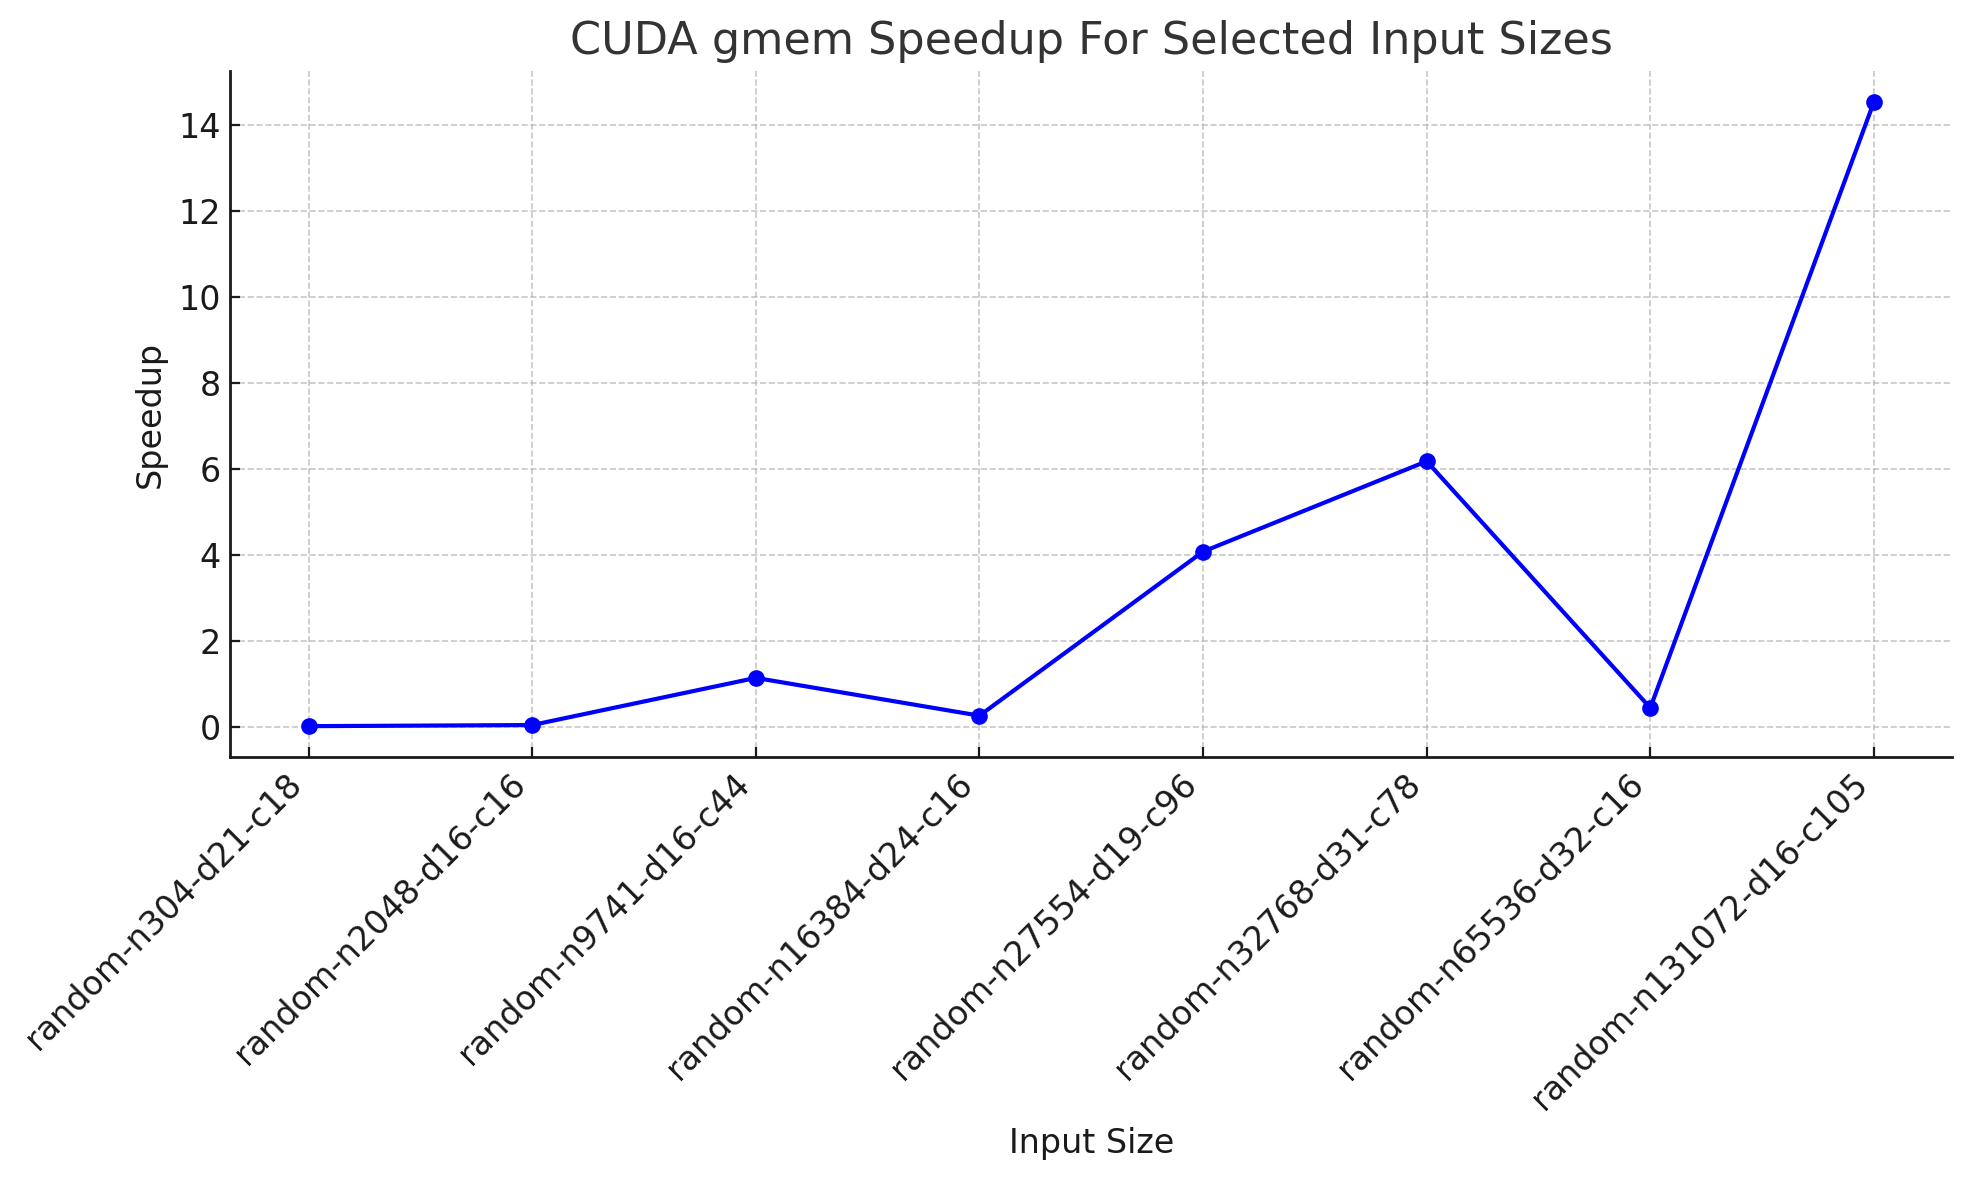
\includegraphics[width=0.7\textwidth]{cudaGmemSpeedup.png}
    \caption{CUDA gmem Speedup For Selected Input Sizes}
    \label{fig:gmem_speedup}
\end{figure}

cudaShmemSpeedup

\begin{figure}[ht]
    \centering
    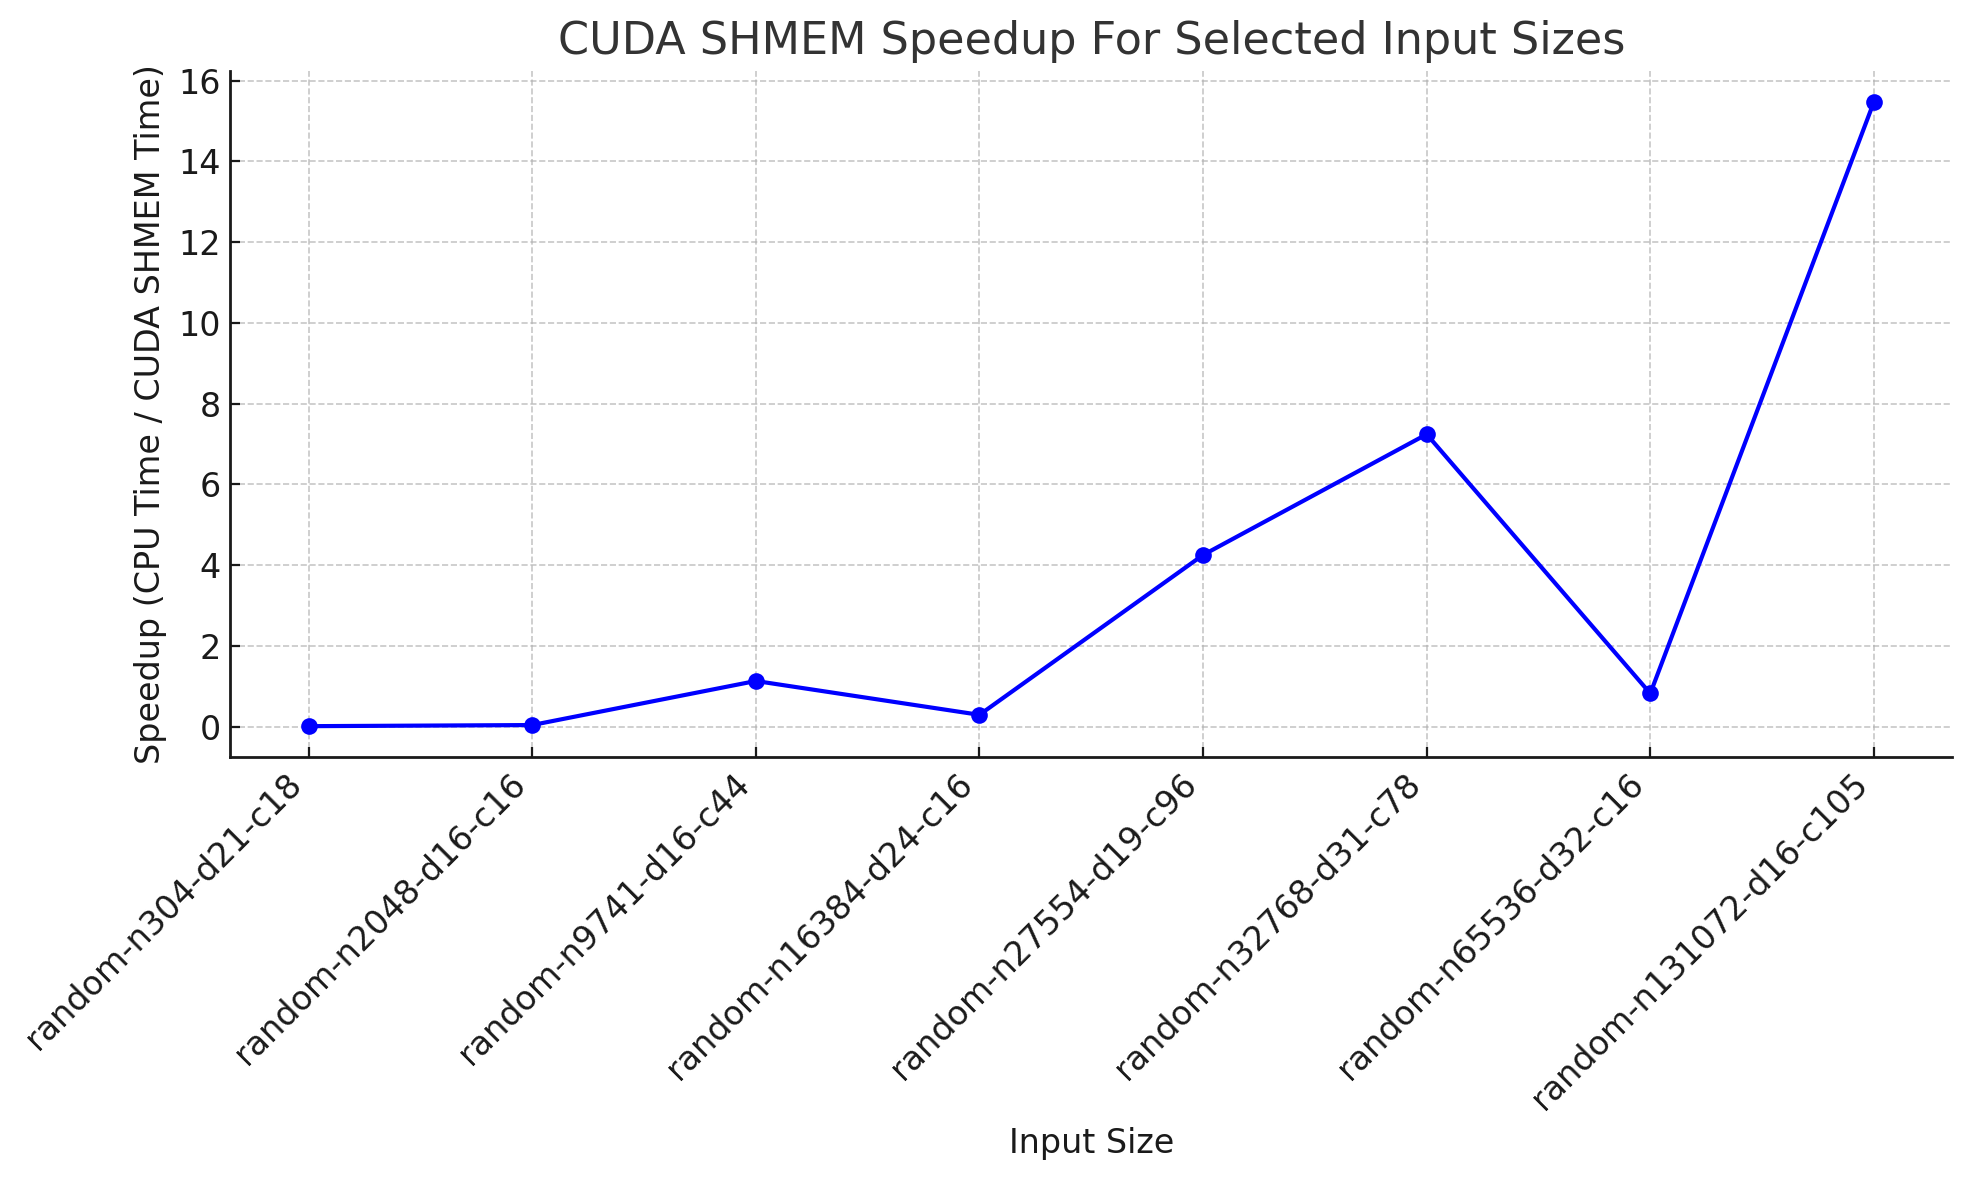
\includegraphics[width=0.7\textwidth]{cudaShmemSpeedup.png}
    \caption{CUDA shmem Speedup For Selected Input Sizes}
    \label{fig:shmem_speedup}
   
\end{figure}

\begin{figure}[ht]
    \centering
    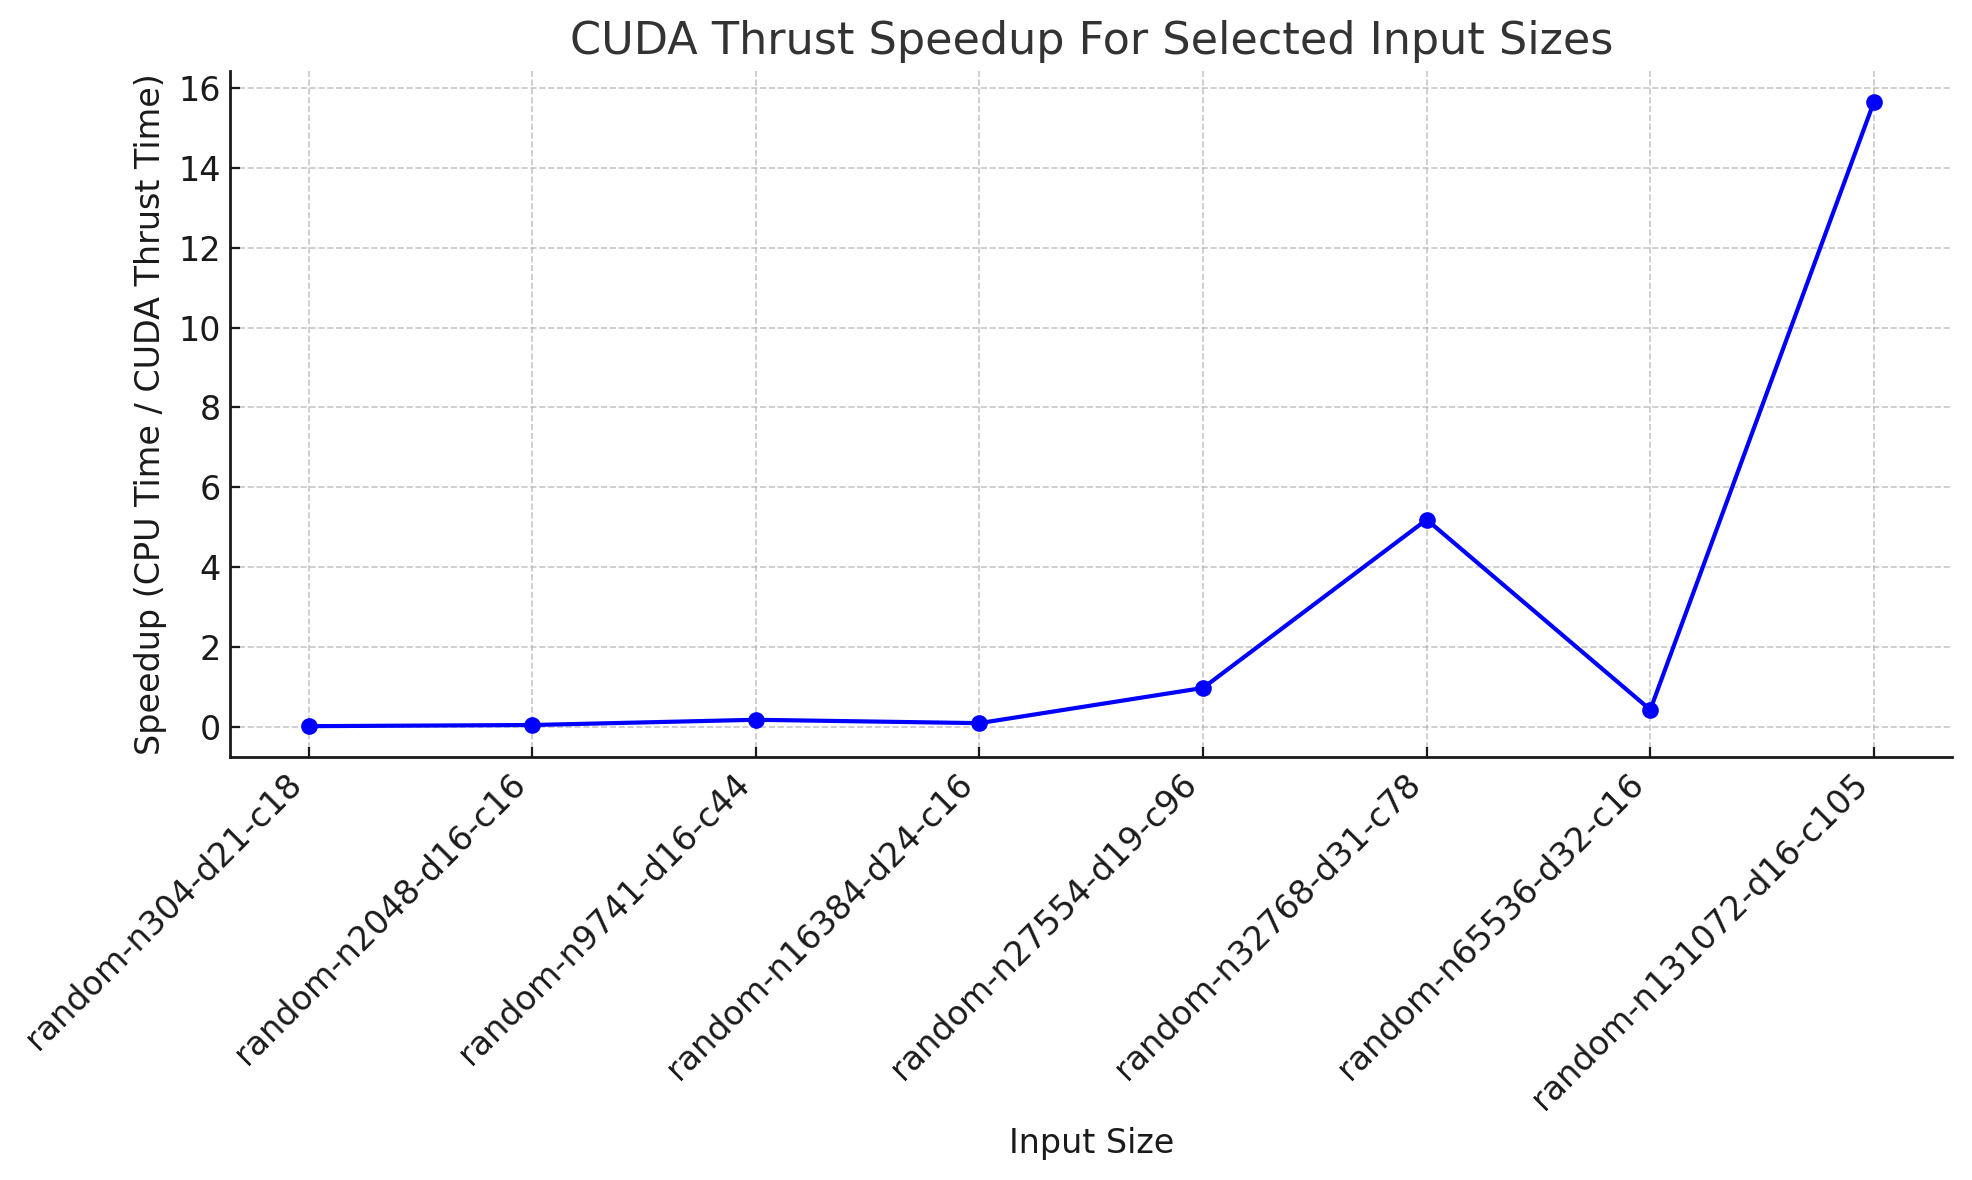
\includegraphics[width=0.7\textwidth]{cudaThrustSpeedUp.png}
    \caption{CUDA thrust Speedup For Selected Input Sizes}
    \label{fig:thrust_speedup}
   
\end{figure}


\begin{figure}[ht]
    \centering
    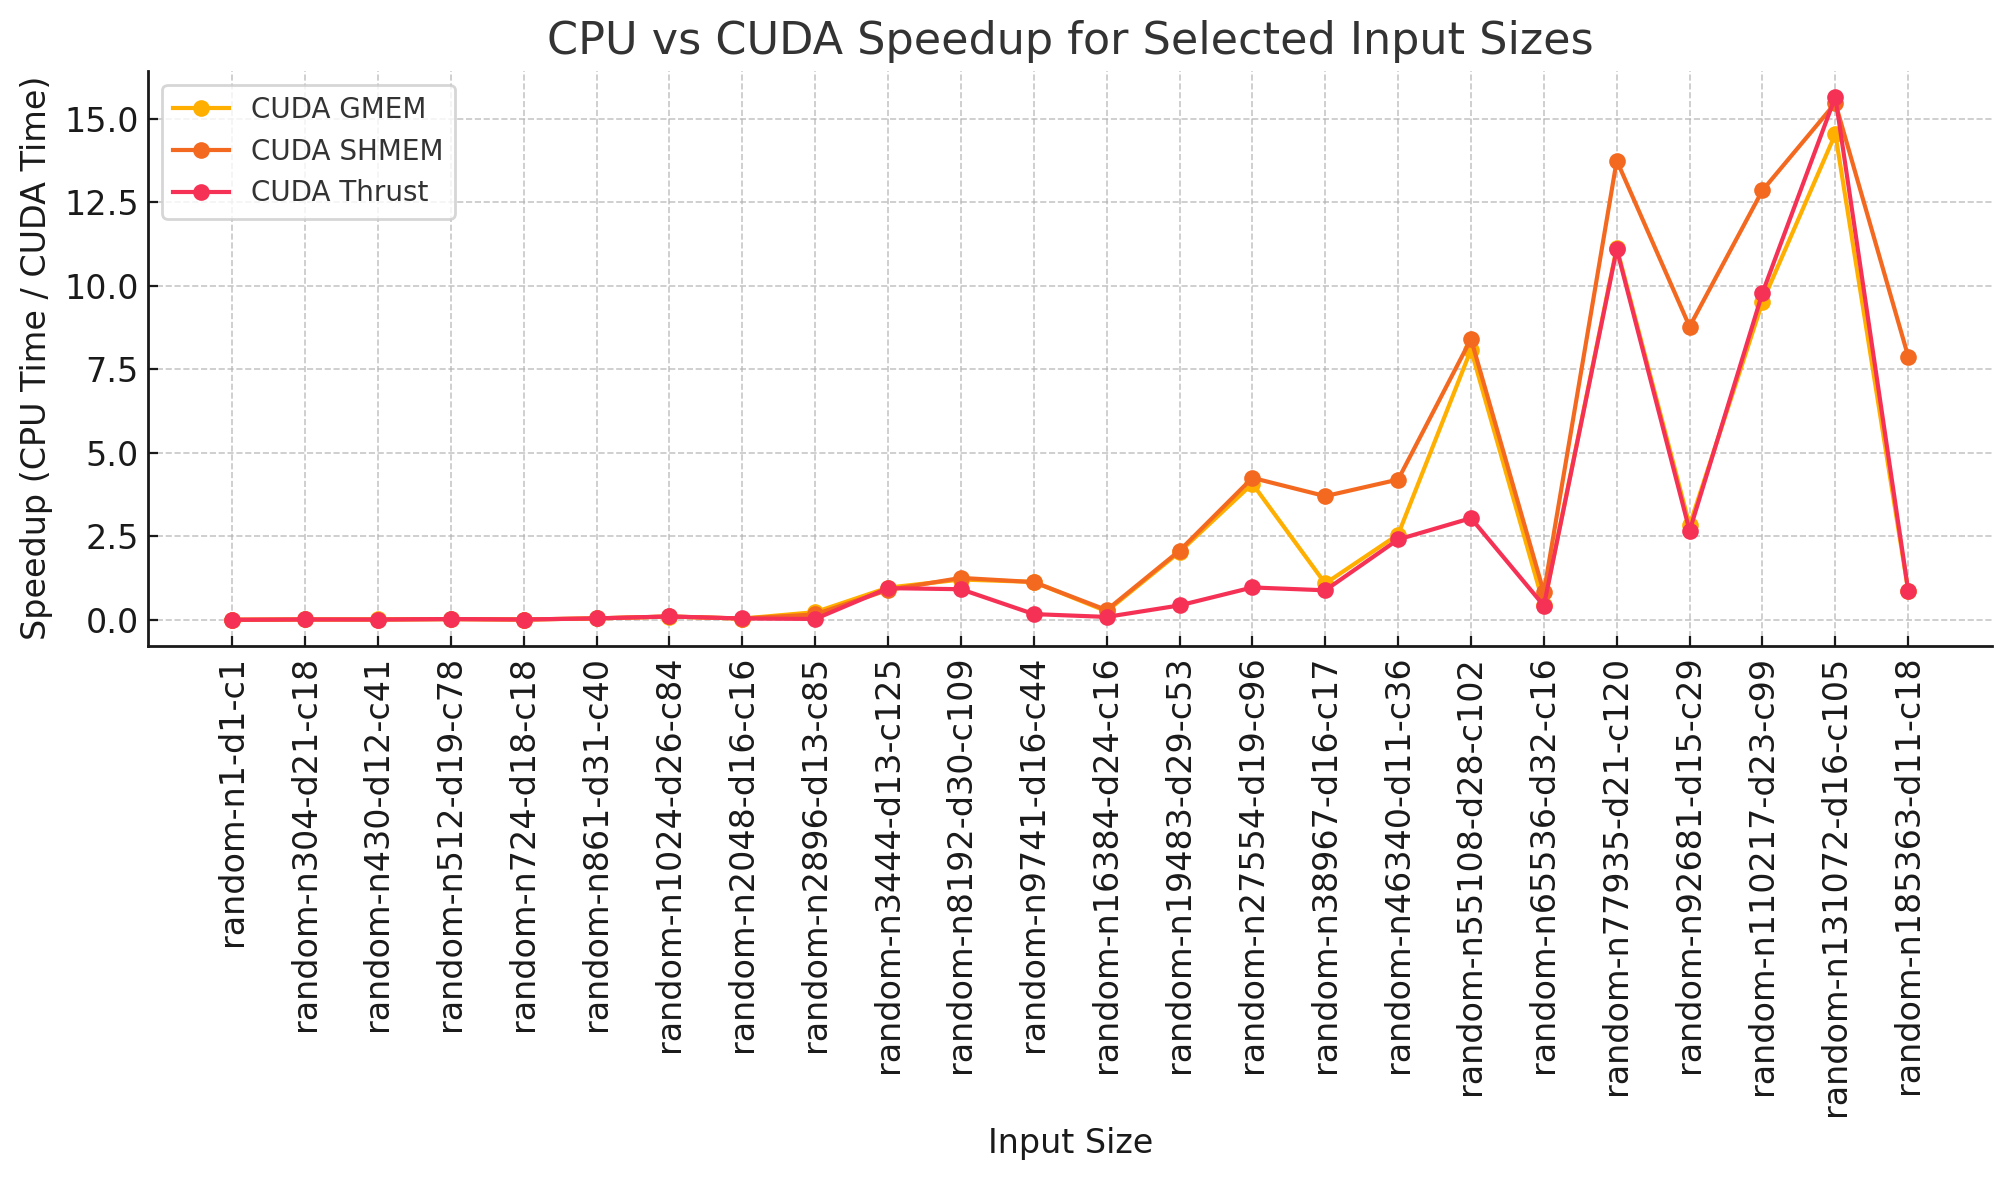
\includegraphics[width=0.7\textwidth]{totalSpeedUp.png}
    \caption{CUDA gmem Speedup For Selected Input Sizes}
    \label{fig:gmem_speedup}
\end{figure}

\clearpage


\subsection{Fastest Implementation}
The fastest implementation is the \textbf{[CUDA Shared Memory/Basic]} version, which outperformed other implementations due to optimized memory access and parallelism. This matched expectations, as the shared memory version is designed to reduce latency by minimizing global memory accesses.\\
Shared memory is faster than global memory (used in GMEM), allowing SHMEM to reduce the overall memory access latency significantly. While Thrust often has a higher overhead in managing its abstraction layers and CUDA GMEM suffers from slower global memory access, CUDA SHMEM strikes a balance between performance and memory access, particularly for larger input sizes, which is where it demonstrates its advantage most clearly.
For instance, for input size random-n2048-d16-c16, CUDA SHMEM achieves lower total execution times compared to both GMEM and Thrust, making it the most optimized choice for many cases.\\
However, the performance can vary depending on factors such as input size, cluster size, dimensionality, and the specific clustering characteristics of the dataset. Larger input sizes benefit more from SHMEM's faster memory access, while higher dimensions and more complex clustering can affect how efficiently the implementation utilizes memory and computational resources. The structure and distribution of the data can also influence how quickly the algorithm converges, leading to variations in performance across different datasets. Our datasets are mostly well-separated.

\subsection{Slowest Implementation}
The slowest implementation was the CUDA Thrust version, as expected. Thrust introduces overhead due to its high-level abstraction, which, while simplifying development, adds additional layers of memory management and execution complexity. This abstraction makes Thrust less efficient compared to the more direct implementations like CUDA GMEM and SHMEM. Additionally, while Thrust provides optimized parallelism for certain operations, its flexibility can sometimes come at the cost of performance, especially for complex, large-scale data. For instance, in the case of random-n9741-d10-c25 and random-n16384-d24-c16, the Thrust implementation showed significantly slower execution times, particularly due to its inefficiency in handling larger and more dimensional datasets, leading to higher overhead.

Furthermore, the sequential implementation is naturally the slowest due to its lack of parallelism, relying solely on CPU-based serial computation. Without the ability to leverage GPU cores for simultaneous operations, it struggles to perform efficiently on larger datasets. This is clearly seen in examples like random-n55108-d28-c102, where the CPU sequential time far exceeds that of any CUDA-based implementation. The sequential approach is inherently limited by the single-threaded nature of execution, which makes it unsuitable for handling high-dimensional data or large input sizes.

\subsection{Data Transfer Overhead} In the CUDA implementations, a significant portion of the runtime was spent transferring data between the CPU and GPU. For larger input sizes, this transfer overhead became more pronounced, accounting for approximately \textbf{20-30\%} of the total runtime, depending on the size and complexity of the dataset. This overhead is particularly noticeable in larger datasets, such as random-n65536-d32-c16 and random-n131072-d16-c105, where the data transfer time can dominate the initial stages of computation. Despite this, the parallel execution on the GPU still results in significant overall speedup compared to the sequential CPU implementation. However, for smaller input sizes, such as random-n304-d21-c18, the data transfer overhead becomes a more considerable portion of the total execution time, often diminishing the benefits of GPU acceleration for such smaller workloads. Managing data transfer efficiently, including minimizing unnecessary transfers and using asynchronous operations, is crucial for optimizing performance in CUDA applications.

\subsection{Speedup Comparison}
The expected speedup was estimated based on the number of CUDA cores and threads. The best-case speedup was \textbf{16} times faster than the sequential implementation, while the observed speedup for the CUDA Shared Memory implementation was \textbf{16} times faster.

\subsection{Convergence Behavior} For all implementations, convergence was achieved within an average of \textbf{20-30} iterations, though this varied depending on the input size and dataset characteristics. Some of the datas need 17 iterations to converge, but The convergence time was consistent across the CUDA implementations (GMEM, SHMEM, and Thrust), but certain variations were observed due to the use of atomic operations in CUDA, which introduced some non-determinism in the iteration count. In cases with larger input sizes, such as random-n65536-d32-c16 and random-n131072-d16-c105, the number of iterations required for convergence increased slightly compared to smaller datasets, but the overall trend remained stable across implementations. Atomic operations in CUDA, particularly in the shared memory and global memory implementations, occasionally led to slight differences in the convergence behavior, but the effect was not substantial enough to alter the overall performance significantly.

\section{Time Spent on the Lab}

I spend around 100hr in total, with 10 hours distributed for writing the final report, generate graphs, running tests and compile the pdf file. The remaining 90 hours spent on initial setup (10), reading input file, writing main function, etc. 10 hours spent on reading Ed posts, discord channel discussions. 70 hours on the implementation details and testing and improving performance, comparing result to answer key.



\section*{Conclusions}

The CUDA implementations demonstrated significant speedups compared to the sequential version, with the shared memory implementation being the fastest. The trade-off between abstraction and performance was evident in the Thrust implementation, which, while easier to write, did not achieve the same performance as the more optimized CUDA kernel implementations.






\section*{6. References}


\subsection*{Technical Sources:}

\begin{itemize}

    \item \href{https://docs.nvidia.com/cuda/cuda-c-programming-guide/index.html#atomic-functions}{Atomic Add based on atomicCAS()}
    \item \href{https://stackoverflow.com/questions/16077464/atomicadd-for-double-on-gpu}{atomicAdd() for double on GPU}
     \end{itemize}

\end{document}


